
早期计算机的编程非常困难,因为处理器慢、内存有限、编译器差劲,完成一个程序需要花费大量的时间。开发者必须知道CPU架构、内存布局,对于当时的编译器,关键的代码必须用汇编来写。

后来情况有所好转了。处理器的速度越来越快,编译器开发者可以使用了一些使程序更快的技巧,所以曾经需要巨大硬盘容量的处理器,现在的所需的容量也就一个普通PC机主存的大小,开发者可以花更多的时间来解决问题,这反映在编程语言和设计风格上。在高级语言和不断发展的设计和编程实践之间,开发者的重点从想在代码中\textbf{说什么},转变为想\textbf{怎么说}。

以前的常识,如CPU到底有多少寄存器,寄存器的名字都是什么,现在却变成了深奥且难懂的话题。曾经的“大型代码库”很难进行管理,而现在已经完全在版本控制系统的掌握之下了。几乎不需要为特定的处理器或内存系统编写特定的代码,可移植的代码已经越来越流行了。

对于手动汇编编程,实际上很难超越编译器生成的代码。当代码量增加,大多数开发者无法完成手动汇编。对于应用程序和编写者来说,有“足够的性能”即可,开发者需要对其他方面的事情更加关注(需要明确的是,开发者可以专注于代码的可读性,而不必担心添加一个名称有意义的函数是否会使程序慢)。

然后,也算是老生常谈,“性能自增长”的时代结束了。看似不断增长的计算能力的提升在程序性能方面……停止了。


\hspace*{\fill} \\ %插入空行
\begin{center}
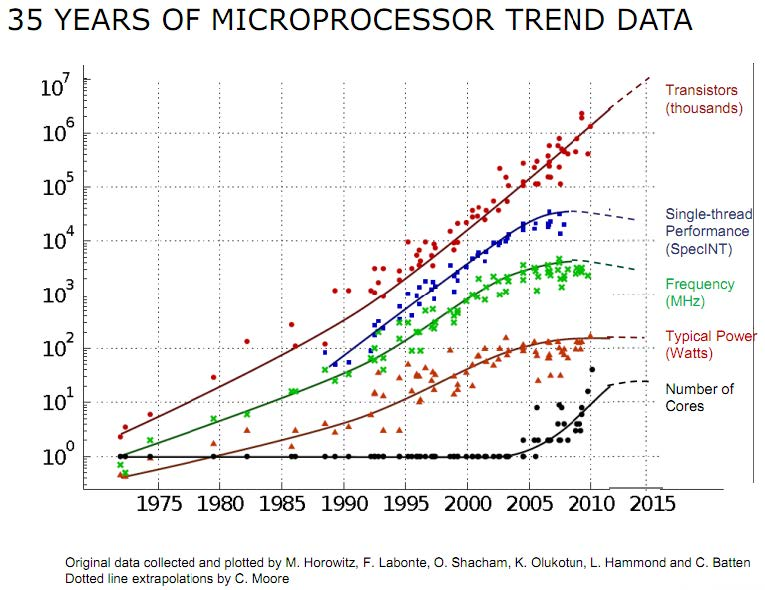
\includegraphics[width=0.9\textwidth]{content/1/chapter1/images/1.jpg}\\
图1.1 -微处理器35年的发展历程 \\
(引用于 \url{https://github.com/karlrupp/microprocessor-trend-data and https://github.com/karlrupp/microprocessor-trend-data/blob/master/LICENSE.txt})
\end{center}

2005年左右,单个CPU的计算能力达到饱和,CPU频率也停止增长。CPU的频率又受到几个因素的限制,其中之一是功耗(如果频率趋势保持不变,如今的CPU每平方毫米的功率将超过将火箭送入太空的大型喷气式发动机)。

从前面的图表中可以明显看出,并不是所有的进步指标都在2005年停滞不前:集成在单个芯片中的晶体管数量一直在增长。那么,如果不是让芯片更快,那是在做什么呢?图表下面的曲线揭示了其中的部分原因。设计师没有将单个处理器做得更大,而是将多个处理器核心放在一起。当然,这些处理器的计算能力会随着核的数量而增加。“晶体管之谜”的第二部分(晶体管都到哪里去了?)中,硬件设计师对处理器功能进行了增强,可以用来提高性能,但也需要开发者了解如何使用。

处理器的变化是并发编程进入主流的原因,但这种变化的意义远不止于此。本书中为了获得最佳性能,开发者需要理解处理器和内存体系结构,及其间的交互,所以出色的性能不再是“偶然获得”。与此同时,在编写代码时所取得的进步,也清楚地表达了需要做什么,而不是如何做。我们仍然希望编写可读和可维护的代码,并且(不是但是)这些代码是高效的。

可以肯定的是,对于许多应用程序来说,现代CPU的性能已经足够,但程序的性能比过去有了更多的关注,这在很大程度上是因为CPU的变化。因为我们想在不一定能获得最佳计算资源的应用程序中,做更多的计算(例如,今天的便携式医疗设备可能有一个神经网络程序在其中工作)。

幸运的是,我们不必在黑暗的储藏室里翻找一堆堆腐烂的穿孔卡片,来重新学习那些古老的艺术形式。任何时候,都有困难的问题,对于许多软件开发者来说,\textit{计算能力永远不够用}这句话完全正确。随着计算能力呈指数级增长,对它的需求也在相应的增长(古老的艺术只会在少数需要它的领域中得以延续)。











